
% \begin{figure}[ht]
%     \centering
%     \begin{subfigure}[t]{0.2\textwidth}
%         \centering
%         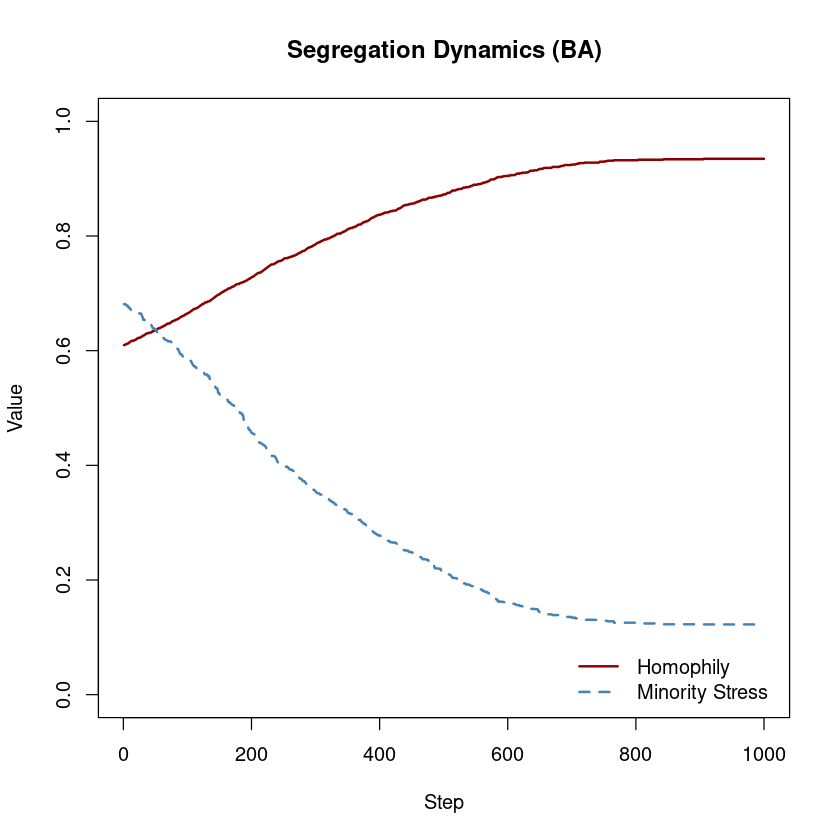
\includegraphics[width=\linewidth]{images/henryba.png}
%         \caption{Caption 1}
%     \end{subfigure}
%     \hfill
%     \begin{subfigure}[t]{0.2\textwidth}
%         \centering
%         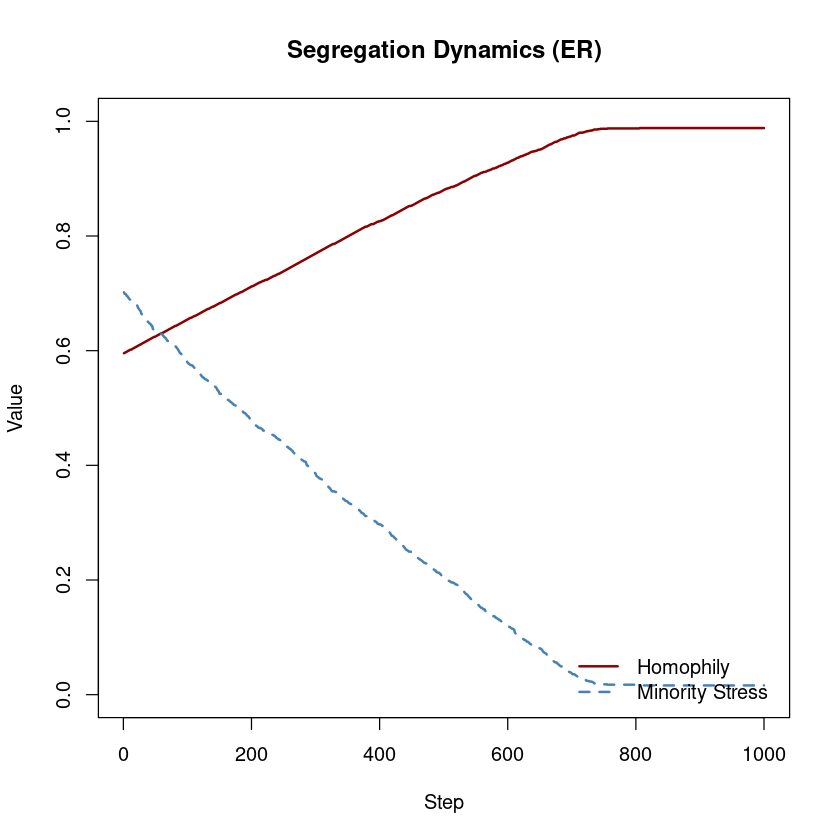
\includegraphics[width=\linewidth]{images/henryer.png}
%         \caption{Caption 2}
%     \end{subfigure}
%     \hfill
%     \begin{subfigure}[t]{0.2\textwidth}
%         \centering
%         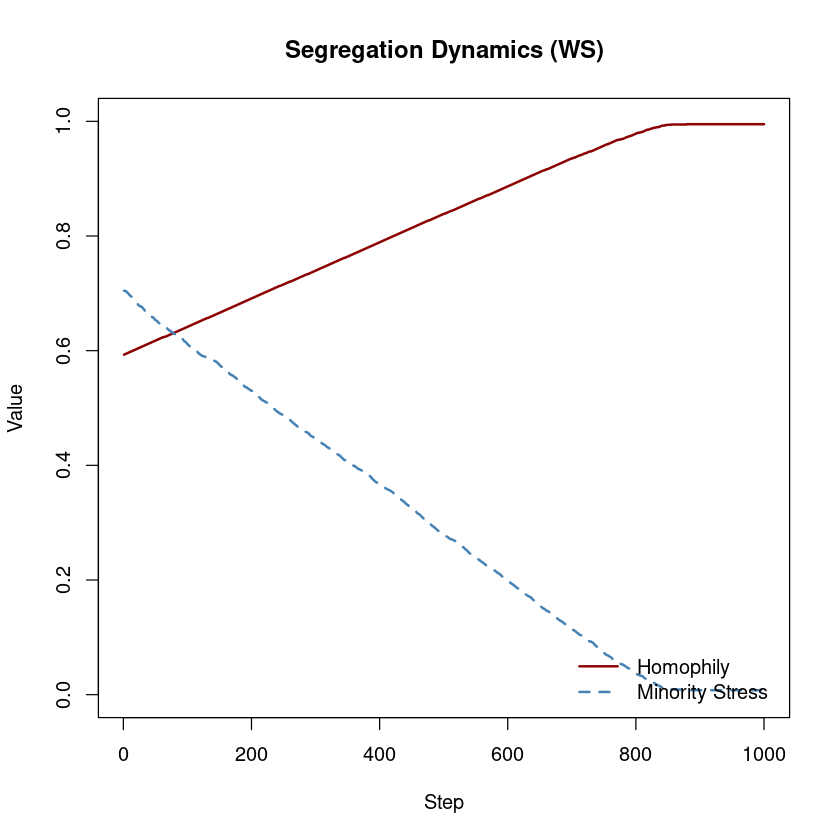
\includegraphics[width=\linewidth]{images/henryws.png}
%         \caption{Caption 3}
%     \end{subfigure}
%     \hfill
%     \begin{subfigure}[t]{0.2\textwidth}
%         \centering
%         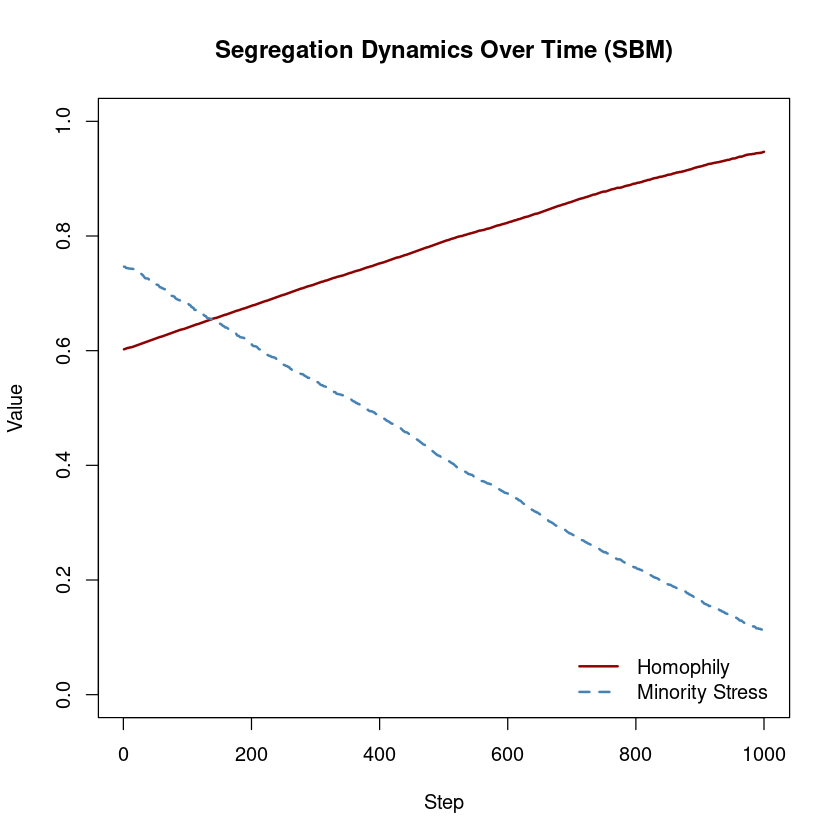
\includegraphics[width=\linewidth]{images/henrysbm.png}
%         \caption{Caption 4}
%     \end{subfigure}
%     \caption{Overall figure caption}
%     \label{fig:henry}
% \end{figure}




\begin{figure}[htbp]
    \centering
    \begin{minipage}[t]{0.24\linewidth}
        \centering
        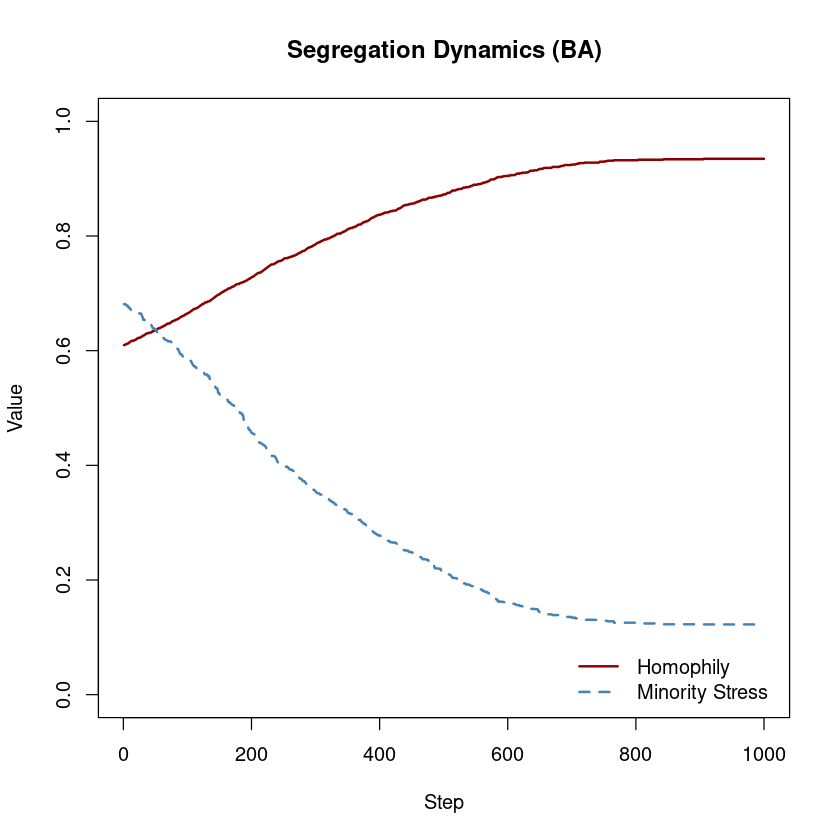
\includegraphics[width=\linewidth]{images/henryba.png}
        \caption{Barabási–Albert}
        \label{fig:henryba}
    \end{minipage}
    \hfill
    \begin{minipage}[t]{0.24\linewidth}
        \centering
        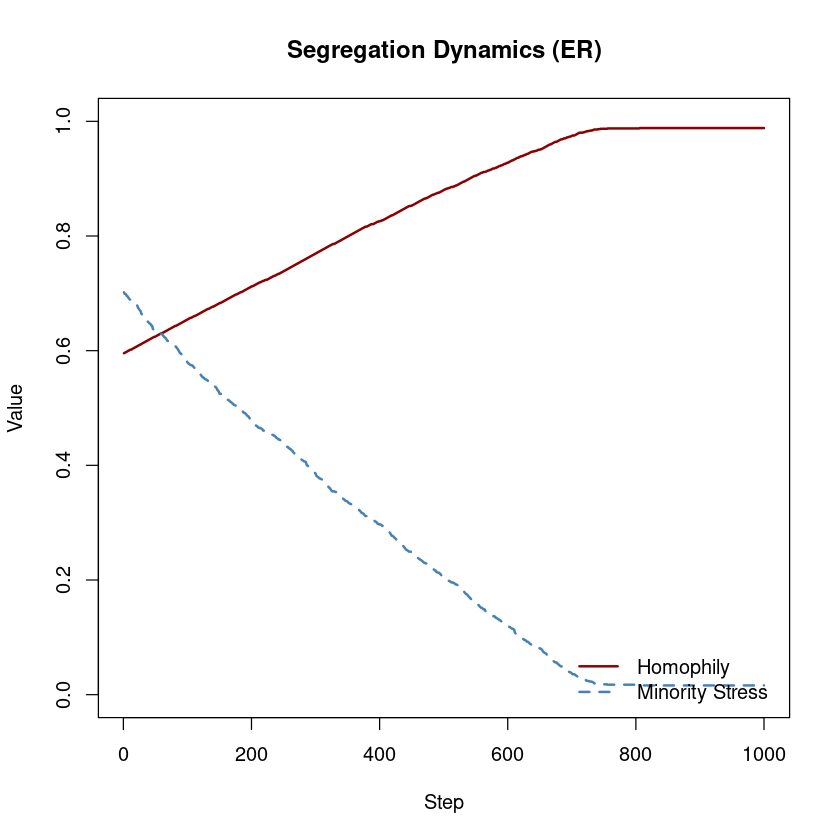
\includegraphics[width=\linewidth]{images/henryer.png}
        \caption{Erdős–Rényi}
        \label{fig:henryer}
    \end{minipage}
    \hfill
    \begin{minipage}[t]{0.24\linewidth}
        \centering
        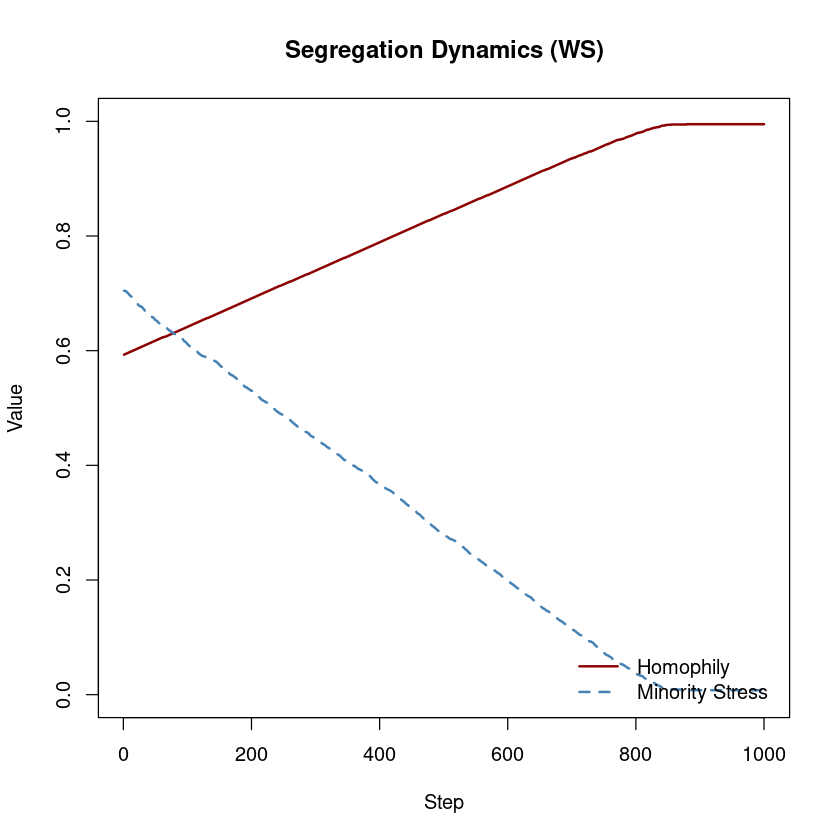
\includegraphics[width=\linewidth]{images/henryws.png}
        \caption{Watts–Strogatz}
        \label{fig:henryws}
    \end{minipage}
    \hfill
    \begin{minipage}[t]{0.24\linewidth}
        \centering
        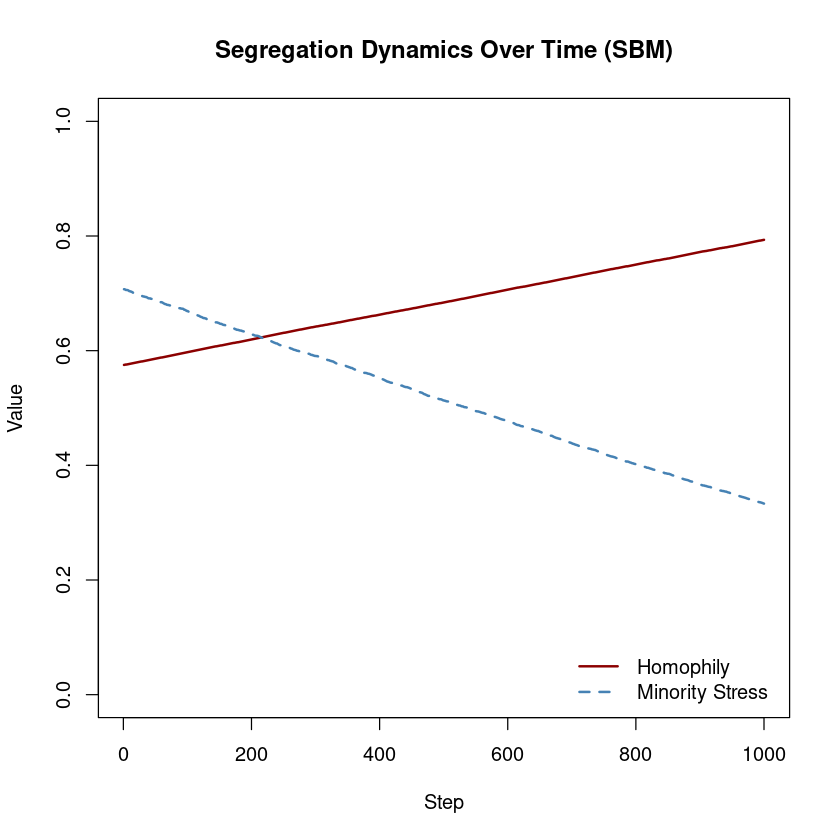
\includegraphics[width=\linewidth]{images/henry2.png}
        \caption{Stochastic Block Model}
        \label{fig:henrysbm}
    \end{minipage}
    \caption{Comparison of network models under the Henry framework.}
    \label{fig:henry_four}
\end{figure}
